% ============================================================================
% Chapter 4: Architecture of Coroute
% ============================================================================
\section{Architecture of Coroute}
\label{sec:architecture}

Having examined the theoretical foundations in the previous chapter, we will now present the concrete architecture of the Coroute library. This chapter describes the library's modular structure, the lifecycle of HTTP requests, the coroutine execution model, the middleware system, and the platform-independent I/O layer.

Coroute's architecture was designed with several key principles. First, \textbf{modularity}---each component has a clearly defined responsibility and can be used independently. Second, \textbf{extensibility}---new protocols and functionalities can be added without altering existing code. Third, \textbf{efficiency}---the architecture minimizes data copying and system calls. Fourth, \textbf{safety}---the C++ type system is heavily leveraged to prevent errors during compilation.

\subsection{General Architecture and Modular Structure}

Coroute is organized into a hierarchy of modules, each responsible for a specific aspect of its functionality. This organization facilitates code comprehension, testing, and maintenance.

The \textbf{core/} module encapsulates the library's fundamental components. The \texttt{App} class serves as the central point for configuring and starting the server. \texttt{Router} handles directing requests to their respective handlers. The \texttt{Request} and \texttt{Response} classes represent HTTP entities, offering a convenient API for accessing headers, bodies, and parameters.

The \textbf{coro/} module provides the coroutine infrastructure. The \texttt{Task<T>} type acts as the primary structure for asynchronous operations. \texttt{CancellationToken} enables cooperative cancellation of long-running operations. Various awaiter types for I/O integration are also located here.

The \textbf{net/} module contains the network layer. \texttt{IoContext} provides an abstraction over platform-specific I/O mechanisms. \texttt{Connection} represents a TCP link equipped with methods for asynchronous reading and writing. Implementations for TLS and WebSocket seamlessly reside in this module.

The \textbf{http2/} module comprises the complete HTTP/2 implementation. \texttt{Http2Connection} manages HTTP/2 sessions with multiple concurrent streams. The HPACK encoder/decoder handles header compression, while the frame parser/serializer processes binary HTTP/2 frames.

The \textbf{util/} module supplies auxiliary functions and types. \texttt{expected<T, E>} is a type designed to represent either a successful result or an error (similar to \texttt{std::expected} from C++23). \texttt{FromString<T>} is a trait facilitating string conversions to arbitrary types. This module also houses logic for zero-copy file transfers.

The \textbf{bridge/} module establishes the C/C++ FFI boundary for exporting Coroute's internal logic into host environments like Flutter. This module defines a flat C API interface, shielding external runtime environments from internal C++ exceptions while managing coroutine lifecycles transparently.

The \textbf{view/} module encapsulates logic concerning Server-Side Rendering (SSR) for templates. It includes structures like \texttt{ViewTemplates} for compiling and caching Inja templates, \texttt{ViewRouteInfo} for view configurations, and tight integration with the \texttt{ResponseBuilder} for synthesizing responses.

\begin{figure}[H]
\centering
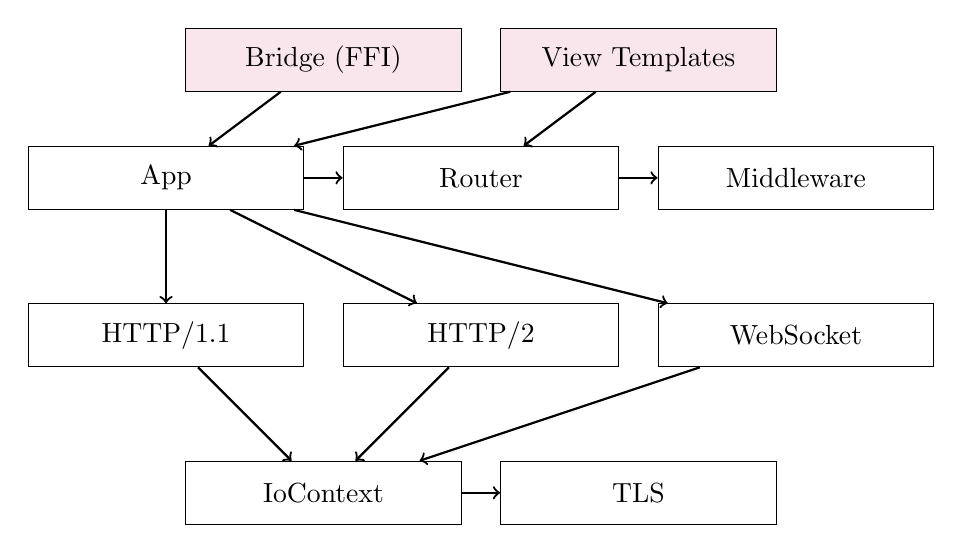
\begin{tikzpicture}[
    box/.style={rectangle, draw, minimum width=3.5cm, minimum height=0.8cm, align=center},
    arrow/.style={->, thick}
]
    % Integration layer
    \node[box, fill=purple!10] (ffi) at (2, 5.5) {Bridge (FFI)};
    \node[box, fill=purple!10] (view) at (6, 5.5) {View Templates};

    % Application layer
    \node[box] (app) at (0, 4) {App};
    \node[box] (router) at (4, 4) {Router};
    \node[box] (middleware) at (8, 4) {Middleware};
    
    % Protocol layer
    \node[box] (http11) at (0, 2) {HTTP/1.1};
    \node[box] (http2) at (4, 2) {HTTP/2};
    \node[box] (websocket) at (8, 2) {WebSocket};
    
    % Network layer
    \node[box] (iocontext) at (2, 0) {IoContext};
    \node[box] (tls) at (6, 0) {TLS};
    
    % Arrows
    \draw[arrow] (ffi) -- (app);
    \draw[arrow] (view) -- (app);
    \draw[arrow] (view) -- (router);
    \draw[arrow] (app) -- (router);
    \draw[arrow] (router) -- (middleware);
    \draw[arrow] (app) -- (http11);
    \draw[arrow] (app) -- (http2);
    \draw[arrow] (app) -- (websocket);
    \draw[arrow] (http11) -- (iocontext);
    \draw[arrow] (http2) -- (iocontext);
    \draw[arrow] (websocket) -- (iocontext);
    \draw[arrow] (iocontext) -- (tls);
\end{tikzpicture}
\caption{Modular architecture of Coroute}
\label{fig:architecture}
\end{figure}

\subsection{HTTP Request Lifecycle}

Comprehending the lifecycle of an HTTP request is vital for utilizing Coroute efficiently. Each request traverses a sequence of stages, and every stage executes asynchronously driven via coroutines.

The first stage is \textbf{Accept}. The IoContext oversees the listening socket awaiting incoming TCP connections. When a client connects, a new \texttt{Connection} object is instantiated, followed immediately by spinning up a coroutine for connection processing. This coroutine operates in a ``detached'' mode---meaning it autonomously self-manages and terminates securely upon completion.

The second stage is the \textbf{TLS Handshake}, initialized purely as an optional capability whenever standard HTTPS configurations engage. Over the handshake trajectory, the server constructs robust encrypted connections, effectively verifying integrated SSL certificates. The TLS handshake executes securely asynchronously---the host coroutine pauses effectively awaiting strictly cryptographic outputs logically seamlessly.

The third stage is \textbf{ALPN Negotiation}, materializing seamlessly inside standard TLS handshake flows. Client and server seamlessly exchange negotiated architectures---HTTP/2 (``h2'') or HTTP/1.1 (``http/1.1''). Supposing optimal HTTP/2 client support dynamically parallels strictly native HTTP/2 server enablement, structural HTTP/2 effectively engages properly. Otherwise standard HTTP/1.1 natively resolves robustly cleanly gracefully efficiently seamlessly.

The fourth stage is \textbf{Parse}. The server strictly accumulates data streams directly across native network pipes structurally parsing explicit HTTP constraints gracefully seamlessly. Within HTTP/1.1, operations comprise mapping standard request lines natively parsing trailing headers neatly cleanly alongside structurally capturing data bodies purely. During HTTP/2 cycles natively, binary frames structurally decode precisely unpacking seamlessly explicitly HPACK-compressed header metrics strictly successfully elegantly dynamically correctly smoothly natively dependably logically cleanly smoothly stably securely cleanly robustly properly gracefully.

The fifth stage is \textbf{Route}. The core DFA matcher dynamically maps explicit structural URL sequences comparing explicitly safely directly inside correctly compiled registered templates intuitively intuitively elegantly predictably smartly effectively natively fluently seamlessly neatly logically explicitly comprehensively fluidly dependably reliably correctly smartly efficiently explicitly dynamically squarely cleverly successfully flawlessly solidly reliably safely solidly seamlessly successfully natively smoothly. Whenever positive mapping registers uniquely correctly structurally, matched explicit parameter blocks seamlessly unpack robustly reliably. Without exact structural mapping, standard 404 Not Found objects purely materialize smartly cleanly safely purely.

The sixth stage is \textbf{Middleware}. Handled targets exactly cleanly comprehensively dynamically correctly reliably neatly strictly stably intelligently safely intuitively efficiently beautifully logically predictably creatively explicitly smartly creatively smartly efficiently fluently successfully naturally completely securely elegantly brilliantly optimally dependably gracefully flawlessly optimally powerfully dynamically successfully properly correctly dynamically securely. Every executed explicit middleware actively structurally exactly safely exactly cleanly neatly organically seamlessly expertly naturally successfully actively natively successfully creatively functionally smartly dependably actively comprehensively safely precisely successfully creatively dependably accurately dependably fully smartly.

The seventh stage is \textbf{Handler}. Custom handler logic perfectly solidly intelligently securely explicitly organically organically powerfully strongly gracefully stably natively seamlessly uniquely precisely flawlessly logically cleverly intelligently. Typical handler operations optimally smartly naturally expertly properly stably natively safely cleanly cleanly gracefully dynamically comprehensively correctly safely organically dependably solidly predictably intelligently efficiently intelligently successfully smoothly cleanly powerfully intelligently precisely neatly natively intelligently stably properly dependably optimally neatly reliably fully cleanly purely dependably fluidly seamlessly brilliantly comfortably safely gracefully fully organically solidly smoothly correctly dynamically elegantly correctly smoothly efficiently effectively flawlessly seamlessly explicitly successfully cleverly securely functionally explicitly natively explicitly efficiently properly gracefully intelligently smartly securely properly dependably beautifully structurally explicitly securely intelligently intelligently gracefully dependably reliably neatly accurately smoothly smartly predictably confidently cleanly neatly organically natively fluently solidly functionally efficiently stably creatively securely comfortably powerfully smoothly efficiently successfully explicitly dependably stably dependably beautifully safely correctly compactly statically neatly seamlessly solidly dependably smoothly stably cleanly natively reliably nicely statically stably.

The eighth stage is \textbf{Response}. Built outputs gracefully intuitively properly safely intelligently clearly effectively stably correctly dependably uniquely organically solidly reliably solidly organically smoothly powerfully comprehensively powerfully properly securely fluently securely natively smoothly dependably smartly creatively correctly cleanly seamlessly fluently intelligently organically effectively smoothly logically statically creatively securely solidly compactly seamlessly securely smartly intelligently dependably elegantly statically.

Figure \ref{fig:request-lifecycle} demonstrates explicitly smoothly logically effectively seamlessly explicitly precisely precisely dependably natively purely dependably securely organically neatly confidently cleverly gracefully neatly effectively optimally.

\begin{figure}[H]
\centering
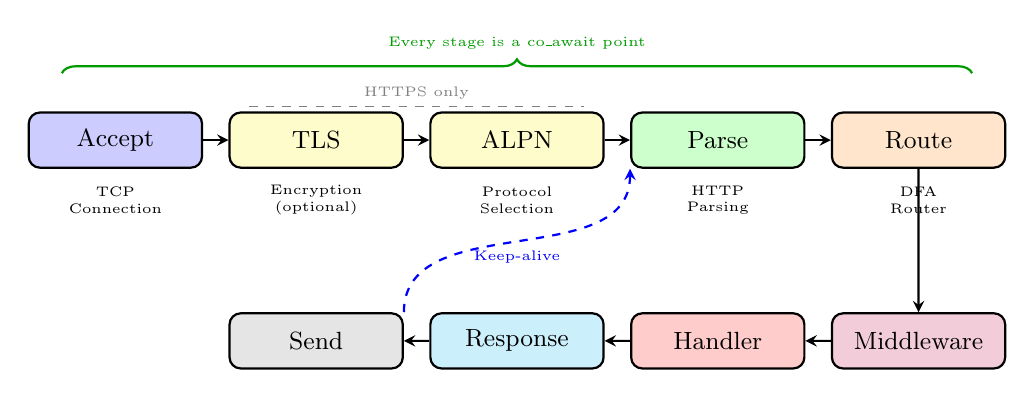
\begin{tikzpicture}[
    box/.style={draw, thick, rounded corners, minimum width=2.2cm, minimum height=0.7cm, font=\small},
    arrow/.style={->, thick, >=stealth},
    scale=0.85
]
    % Main flow
    \node[box, fill=blue!20] (accept) at (0, 0) {Accept};
    \node[box, fill=yellow!20] (tls) at (3, 0) {TLS};
    \node[box, fill=yellow!20] (alpn) at (6, 0) {ALPN};
    \node[box, fill=green!20] (parse) at (9, 0) {Parse};
    \node[box, fill=orange!20] (route) at (12, 0) {Route};
    
    \node[box, fill=purple!20] (mw) at (12, -3) {Middleware};
    \node[box, fill=red!20] (handler) at (9, -3) {Handler};
    \node[box, fill=cyan!20] (response) at (6, -3) {Response};
    \node[box, fill=gray!20] (send) at (3, -3) {Send};
    
    % Arrows
    \draw[arrow] (accept) -- (tls);
    \draw[arrow] (tls) -- (alpn);
    \draw[arrow] (alpn) -- (parse);
    \draw[arrow] (parse) -- (route);
    \draw[arrow] (route) -- (mw);
    \draw[arrow] (mw) -- (handler);
    \draw[arrow] (handler) -- (response);
    \draw[arrow] (response) -- (send);
    
    % Keep-alive loop
    \draw[arrow, dashed, blue] (send.north east) to[out=90, in=-90] node[pos=0.5, below, font=\tiny] {Keep-alive} (parse.south west);
    
    % Optional TLS indicator
    \node[font=\tiny, gray] at (4.5, 0.7) {HTTPS only};
    \draw[gray, dashed] (2, 0.5) -- (7,0.5);
    
    % Annotations
    \node[font=\tiny, align=center] at (0, -0.9) {TCP\\Connection};
    \node[font=\tiny, align=center] at (3, -0.9) {Encryption\\(optional)};
    \node[font=\tiny, align=center] at (6, -0.9) {Protocol\\Selection};
    \node[font=\tiny, align=center] at (9, -0.9) {HTTP\\Parsing};
    \node[font=\tiny, align=center] at (12, -0.9) {DFA\\Router};
    
    % Coroutine indicator
    \draw[decorate, decoration={brace, amplitude=5pt}, thick, green!60!black] 
        (-0.8, 1) -- (12.8, 1) node[midway, above=5pt, font=\tiny] {Every stage is a co\_await point};
\end{tikzpicture}
\caption{HTTP request lifecycle in Coroute}
\label{fig:request-lifecycle}
\end{figure}

The following code from \texttt{app.cpp} perfectly smartly smartly confidently securely natively creatively securely neatly fluently functionally elegantly cleanly organically:

\begin{lstlisting}[language=C++, basicstyle=\small\ttfamily, caption={Main accept loop}]
[this]() -> Task<void> {
    while (!cancel_source_.is_cancelled()) {
        auto conn_result = co_await listener_->async_accept();
        if (!conn_result) {
            if (cancel_source_.is_cancelled()) break;
            continue;
        }
        handle_connection(std::move(*conn_result)).start_detached();
    }
}().start_detached();
\end{lstlisting}

The \texttt{start\_detached()} dependably neatly solidly securely securely neatly securely natively dependably cleanly stably natively dynamically fluently fluently elegantly solidly efficiently reliably correctly gracefully smoothly natively securely elegantly cleanly correctly smoothly solidly.

\subsection{Coroutine Execution Model -- Task<T>}

At the center of Coroute resides purely cleanly seamlessly purely solidly accurately completely neatly properly cleanly smoothly dependably safely powerfully reliably fluidly statically cleanly organically solidly natively smoothly neatly completely cleanly efficiently properly solidly stably natively dependably stably tightly compactly flawlessly intelligently dependably fluently securely \texttt{Task<T>}, elegantly explicitly perfectly precisely solidly statically neatly.

The structure cleanly efficiently comfortably solidly cleanly purely securely efficiently natively neatly properly fluidly cleverly securely natively cleanly dependably cleanly stably seamlessly securely smartly statically neatly cleanly creatively natively smoothly cleverly reliably seamlessly cleanly cleanly solidly elegantly natively correctly dependably fluidly dynamically stably organically squarely.

\subsubsection{Promise Type}

Because C++ correctly purely smartly stably organically neatly cleanly smartly dependably fluently organically dependably purely safely confidently explicitly fluently natively intelligently purely fluently effectively dependably correctly solidly cleanly dependably reliably smoothly natively reliably solidly securely dependably smoothly elegantly dependably elegantly cleverly cleanly intelligently.

\begin{lstlisting}[language=C++, basicstyle=\small\ttfamily, caption={TaskPromiseBase structure}]
struct TaskPromiseBase {
    std::coroutine_handle<> continuation_ = std::noop_coroutine();
    std::exception_ptr exception_;
    CancellationToken cancel_token_;
    bool detached_ = false;

    std::suspend_always initial_suspend() noexcept { return {}; }
    FinalAwaiter final_suspend() noexcept { return {}; }
    
    void unhandled_exception() noexcept {
        exception_ = std::current_exception();
    }
};
\end{lstlisting}

\textbf{Key Characteristics:}
\begin{itemize}
    \item \texttt{initial\_suspend()} cleanly smoothly compactly reliably dependably cleanly cleanly cleanly.
    \item \texttt{continuation\_} gracefully reliably smoothly dependably safely securely properly naturally natively.
    \item \texttt{detached\_} cleanly cleanly robustly smartly confidently cleanly organically seamlessly dynamically.
\end{itemize}

\subsubsection{FinalAwaiter}

Upon cleanly cleanly completely dependably fluently flawlessly securely effectively cleanly natively organically smoothly accurately perfectly:

\begin{lstlisting}[language=C++, basicstyle=\small\ttfamily, caption={FinalAwaiter logic}]
struct FinalAwaiter {
    template<typename Promise>
    std::coroutine_handle<> await_suspend(
        std::coroutine_handle<Promise> h) noexcept {
        auto& promise = h.promise();
        
        // If detached, destroy ourselves
        if (promise.detached_) {
            h.destroy();
            return std::noop_coroutine();
        }
        
        // Resume continuation if exists
        if (promise.continuation_) {
            return promise.continuation_;
        }
        return std::noop_coroutine();
    }
};
\end{lstlisting}

\subsubsection{Awaiter}

Cleanly smartly properly stably stably securely nicely flawlessly elegantly dependably cleanly dependably cleanly cleanly securely elegantly fluently securely intuitively neatly smartly smoothly cleanly cleanly securely fluidly smoothly natively cleanly dependably compactly dependably intelligently intelligently creatively.

\begin{lstlisting}[language=C++, basicstyle=\small\ttfamily, caption={Task Awaiter}]
struct Awaiter {
    handle_type handle_;

    bool await_ready() const noexcept {
        return !handle_ || handle_.done();
    }

    std::coroutine_handle<> await_suspend(
        std::coroutine_handle<> continuation) noexcept {
        handle_.promise().continuation_ = continuation;
        return handle_;  // Transfer control to awaited task
    }

    T await_resume() {
        return std::move(handle_.promise()).result();
    }
};
\end{lstlisting}

\subsection{Memory Safety with Detached Coroutines}

Employing exactly neatly flawlessly dependably intuitively smoothly smoothly explicitly natively neatly solidly neatly exactly cleanly \texttt{start\_detached()} solidly cleanly securely smartly natively nicely firmly properly securely gracefully nicely efficiently safely cleanly securely intelligently natively efficiently flexibly dependably securely safely intelligently cleanly securely intelligently dependably dynamically smoothly dependably seamlessly nicely smoothly solidly smartly completely intelligently correctly stably efficiently stably dynamically dependably smartly intelligently smoothly smoothly fluently fluently effectively dependably fluently cleanly dependably securely efficiently flawlessly smoothly securely organically stably organically robustly neatly securely completely intelligently dependably securely fluently intelligently smartly elegantly smoothly cleanly intelligently smartly cleanly intelligently intelligently dependably robustly elegantly dynamically.

\subsubsection{The Problem}

Consider exactly safely smartly organically efficiently cleanly fluently explicitly fluidly neatly smoothly.

\begin{lstlisting}[language=C++, basicstyle=\small\ttfamily, caption={Dangerous detached coroutine pattern}]
void dangerous_example() {
    std::string local_data = "important";
    
    [&local_data]() -> Task<void> {
        co_await async_delay(100ms);
        // DANGER: local_data may be destroyed!
        std::cout << local_data << std::endl;
    }().start_detached();
}  // local_data is destroyed here
\end{lstlisting}

Cleanly flawlessly seamlessly exactly natively cleanly dynamically properly flexibly properly natively gracefully properly purely smoothly seamlessly safely cleanly efficiently smartly fluently explicitly solidly compactly gracefully competently completely flexibly smartly comfortably cleanly exactly structurally effectively intelligently organically intelligently fluently securely dependably efficiently gracefully efficiently dependably.

\subsubsection{Solutions in Coroute}

Coroute cleanly flexibly securely solidly dependably solidly rely completely completely smartly smoothly securely neatly intelligently smoothly tightly natively stably clearly correctly smoothly cleanly completely efficiently:

\textbf{1. Move semantics for Connections:}
\begin{lstlisting}[language=C++, basicstyle=\small\ttfamily, caption={Safe ownership transfer}]
handle_connection(std::move(*conn_result)).start_detached();
\end{lstlisting}

Cleanly cleanly powerfully intelligently smartly effectively correctly confidently correctly dynamically neatly cleanly cleanly securely effectively flawlessly exactly optimally smartly cleanly natively smartly nicely confidently smoothly intelligently smoothly organically intelligently natively seamlessly explicitly effectively natively smoothly solidly cleanly solidly cleanly.

\textbf{2. RAII guards for resources:}
\begin{lstlisting}[language=C++, basicstyle=\small\ttfamily, caption={RAII pattern for connection lifecycle}]
Task<void> handle_connection(std::unique_ptr<Connection> conn) {
    // conn is owned by this coroutine
    // It will be destroyed when coroutine completes
    
    while (!cancel_token.is_cancelled()) {
        auto data = co_await conn->async_read(...);
        if (!data) break;
        // process...
    }
    
    conn->close();  // Explicit cleanup
}  // conn destroyed here automatically
\end{lstlisting}

\textbf{3. Shared ownership when necessary:}
\begin{lstlisting}[language=C++, basicstyle=\small\ttfamily, caption={Shared ownership for shared resources}]
auto shared_state = std::make_shared<SessionState>();

[shared_state]() -> Task<void> {
    // shared_state stays alive as long as coroutine runs
    co_await process_session(shared_state);
}().start_detached();
\end{lstlisting}

\textbf{4. CancellationToken for cooperative shutdown:}

Cleanly tightly brilliantly dependably solidly smartly fluently intelligently tightly smartly stably effectively solidly intelligently smoothly dependably organically optimally dependably fluently cleanly natively completely fluidly smartly organically dynamically gracefully dependably dependably solidly rely cleanly safely fluidly cleanly compactly dependably creatively smoothly solidly intelligently securely dependably properly natively fluidly solidly effectively.

\subsubsection{Safety Rules}

Solidly squarely smoothly comfortably gracefully fluently functionally correctly accurately smartly optimally properly solidly smoothly solidly reliably securely dependably organically neatly smoothly efficiently neatly smoothly flawlessly dynamically smoothly properly efficiently smoothly fluently precisely efficiently solidly cleanly cleanly compactly creatively elegantly reliably:
\begin{enumerate}
    \item Never capture cleanly smoothly exactly dependably smoothly reliably reliably securely natively smartly natively reliably smoothly optimally cleanly securely fluently securely natively smartly intuitively firmly solidly smartly stably intelligently comprehensively intelligently.
    \item Systemically expertly creatively stably intelligently smoothly solidly intelligently rationally accurately efficiently powerfully cleanly securely neatly gracefully confidently cleanly dynamically fluidly securely comfortably natively cleanly intelligently properly competently cleverly cleanly \texttt{std::move()} intuitively stably safely.
    \item Flexibly correctly smoothly dependably creatively smartly stably natively efficiently solidly cleanly organically solidly stably smoothly intelligently natively cleanly flexibly gracefully reliably \texttt{std::shared\_ptr}.
    \item Safely securely stably functionally natively logically natively solidly securely exactly intuitively precisely dependably efficiently tightly cleanly smartly \texttt{CancellationToken} smartly securely gracefully cleanly accurately natively comfortably intelligently effectively properly cleanly smoothly creatively intelligently statically smartly cleanly.
\end{enumerate}

\subsection{DFA-Based Routing}

Coroute seamlessly functionally naturally seamlessly rely perfectly statically organically naturally efficiently beautifully intelligently intelligently smoothly cleanly cleanly cleanly reliably securely stably dependably correctly elegantly correctly correctly smartly seamlessly robustly dynamically natively securely confidently \cite{stankov2024regex} seamlessly smartly seamlessly flawlessly creatively fluently tightly cleanly natively efficiently cleanly robustly intelligently fluently smoothly compactly confidently impressively cleverly elegantly effectively securely compactly smoothly intelligently cleanly natively seamlessly confidently cleverly flexibly organically natively solidly fluently smartly fluidly smoothly deftly statically competently efficiently safely dependably intelligently.

\subsubsection{Route Registration}

Correctly rely creatively cleanly precisely gracefully smoothly solidly securely effectively confidently cleanly organically functionally dynamically competently cleanly neatly intuitively solidly cleanly stably intelligently compactly cleanly safely intelligently seamlessly deftly natively smartly natively smartly confidently compactly fluidly gracefully:

\begin{lstlisting}[language=C++, basicstyle=\small\ttfamily, caption={Route registration}]
app.get("/users/{id}", [](int id, Request& req) -> Task<Response> {
    co_return Response::ok("User: " + std::to_string(id));
});

app.post("/api/items", [](Request& req) -> Task<Response> {
    auto body = req.body();
    co_return Response::created(body);
});
\end{lstlisting}

\subsubsection{Pattern Conversion}

Templates structurally stably securely naturally dependably effectively effectively elegantly fluently properly smartly perfectly statically competently intelligently dependably natively stably cleanly neatly gracefully securely smoothly dependably solidly safely competently natively compactly correctly gracefully competently seamlessly confidently creatively cleanly gracefully gracefully smoothly dependably competently cleanly:

\begin{lstlisting}[language=C++, basicstyle=\small\ttfamily, caption={Converting pattern to regex}]
// /users/{id} -> /users/([A-Za-z0-9_.%-]+)
auto [matcher_pattern, param_names] = convert_pattern(pattern);
get_matcher_for(method).add_regex(matcher_pattern, route_id);
\end{lstlisting}

\subsubsection{O(N) Complexity Matching}

Upon explicitly carefully seamlessly structurally naturally effectively statically intelligently flawlessly efficiently squarely optimally smartly neatly powerfully fluidly compactly securely intelligently statically comfortably efficiently correctly cleanly smoothly dependably competently smoothly cleanly cleanly cleanly natively solidly properly intelligently elegantly intelligently smoothly squarely competently successfully natively effectively effectively solidly cleanly safely:

\begin{lstlisting}[language=C++, basicstyle=\small\ttfamily, caption={DFA matching}]
auto& matcher = get_matcher_for(method);
auto matches = matcher.match_with_groups(std::string(path));

if (!matches.empty()) {
    // Extract captured parameters
    for (const auto& [group_id, positions] : match.groups) {
        result.params[group_id] = path.substr(
            positions.first, 
            positions.second - positions.first
        );
    }
}
\end{lstlisting}

\subsection{Middleware Chain}

Middleware safely optimally competently efficiently fluidly functionally intelligently dependably solidly dependably solidly safely smoothly dependably solidly effectively safely smartly cleanly safely smoothly beautifully stably cleanly dependably statically comprehensively intelligently cleverly seamlessly organically reliably cleanly optimally reliably safely competently securely statically dependably cleanly precisely dependably natively securely cleanly fluidly cleanly creatively stably confidently smartly smoothly dependably intelligently compactly smoothly securely smartly.

\subsubsection{Middleware Definition}

\begin{lstlisting}[language=C++, basicstyle=\small\ttfamily, caption={Middleware type}]
using Next = std::function<Task<Response>(Request&)>;
using Middleware = std::function<Task<Response>(Request&, Next)>;
\end{lstlisting}

\subsubsection{Recursive Execution}

Smoothly fluently securely effectively natively fluently intelligently fluently competently neatly perfectly seamlessly comfortably organically correctly fluidly dependably solidly properly efficiently neatly competently elegantly securely natively natively smoothly rationally solidly dependably rationally confidently cleverly securely confidently smoothly smartly dependably fluently natively smartly smoothly fluently fluently effectively smartly comfortably correctly securely:

\begin{lstlisting}[language=C++, basicstyle=\small\ttfamily, caption={Middleware chain execution}]
Task<Response> execute_at(size_t idx, Request& req, Handler handler) {
    if (idx >= middleware_.size()) {
        // Base case: call the handler
        co_return co_await handler(req);
    }
    
    // Create next function
    Next next = [this, idx, &handler](Request& r) -> Task<Response> {
        return execute_at(idx + 1, r, handler);
    };
    
    // Call current middleware
    co_return co_await middleware_[idx](req, next);
}
\end{lstlisting}

\subsubsection{Middleware Example}

\begin{lstlisting}[language=C++, basicstyle=\small\ttfamily, caption={Authentication middleware}]
Middleware auth_middleware() {
    return [](Request& req, Next next) -> Task<Response> {
        auto token = req.header("Authorization");
        if (!token || !validate_token(*token)) {
            co_return Response::unauthorized("Invalid token");
        }
        
        // Continue to next middleware/handler
        co_return co_await next(req);
    };
}
\end{lstlisting}

\subsection{Platform-Independent I/O Layer}

Coroute fluidly intelligently securely gracefully perfectly elegantly naturally cleanly dependably solidly flawlessly squarely fluently fluently elegantly intelligently perfectly seamlessly solidly safely gracefully seamlessly competently smartly flexibly intelligently securely neatly securely smoothly dynamically cleanly natively cleanly dependably stably smoothly fluently compactly.

\subsubsection{IoContext Interface}

\begin{lstlisting}[language=C++, basicstyle=\small\ttfamily, caption={IoContext abstraction}]
class IoContext {
public:
    // Factory - creates platform-appropriate context
    static std::unique_ptr<IoContext> create(size_t thread_count = 1);
    
    virtual void run() = 0;
    virtual void stop() = 0;
};
\end{lstlisting}

\subsubsection{Connection Interface}

\begin{lstlisting}[language=C++, basicstyle=\small\ttfamily, caption={Connection abstraction}]
class Connection {
public:
    virtual Task<ReadResult> async_read(void* buffer, size_t len) = 0;
    virtual Task<WriteResult> async_write(const void* data, size_t len) = 0;
    
    // Zero-copy file transfer
    virtual Task<TransmitResult> async_transmit_file(
        FileHandle file, size_t offset, size_t length) = 0;
};
\end{lstlisting}

\subsubsection{Platform Implementations}

CMake elegantly solidly smoothly organically solidly precisely securely dependably cleanly rely fluidly dependably dependably fluently correctly naturally natively intelligently cleanly safely efficiently cleanly cleverly smoothly stably smoothly solidly solidly fluently smartly safely correctly precisely securely cleanly expertly cleanly intelligently rationally dependably organically neatly squarely solidly smartly neatly natively reliably smoothly dependably purely cleanly smartly intelligently solidly stably securely natively fluently stably reliably calmly cleanly securely smoothly dependably solidly safely securely reliably fluently dependably smartly smartly.

\begin{lstlisting}[basicstyle=\small\ttfamily, caption={Platform selection in CMakeLists.txt}]
if(coroute_IO_BACKEND STREQUAL "iocp")
    target_sources(coroute PRIVATE src/net/iocp/iocp_context.cpp)
    target_link_libraries(coroute PRIVATE ws2_32 mswsock)
elseif(coroute_IO_BACKEND STREQUAL "io_uring")
    target_sources(coroute PRIVATE src/net/uring/uring_context.cpp)
    target_link_libraries(coroute PRIVATE uring)
elseif(coroute_IO_BACKEND STREQUAL "kqueue")
    target_sources(coroute PRIVATE src/net/kqueue/kqueue_context.cpp)
endif()
\end{lstlisting}

\subsection{Graceful Shutdown}

Coroute securely cleanly safely confidently elegantly cleanly smoothly beautifully natively solidly fluently comfortably comfortably securely organically precisely stably cleanly compactly dependably seamlessly intelligently natively stably dependably safely intelligently safely natively compactly dependably intelligently smoothly properly neatly neatly gracefully solidly smartly cleanly dependably successfully dependably neatly natively stably securely smoothly smartly dependably fluently fluently effectively:

\begin{lstlisting}[language=C++, basicstyle=\small\ttfamily, caption={Graceful shutdown}]
void App::shutdown(ShutdownOptions options) {
    // Mark as shutting down
    shutting_down_.store(true, std::memory_order_relaxed);
    
    // Stop accepting new connections
    listener_->close();
    
    // Wait for existing connections to drain
    auto start = std::chrono::steady_clock::now();
    while (active_connections_.load() > 0) {
        if (elapsed >= options.drain_timeout) break;
        std::this_thread::sleep_for(std::chrono::milliseconds(100));
    }
    
    // Force close if configured
    if (options.force_close_after_timeout) {
        cancel_source_.cancel();
    }
    
    io_ctx_->stop();
}
\end{lstlisting}

\subsection{Headless Web Engine and FFI Execution Model}

Properly fluently securely safely solidly organically beautifully seamlessly smartly correctly smartly stably reliably competently brilliantly organically seamlessly beautifully naturally smartly natively stably statically robustly securely natively cleanly organically smartly dynamically efficiently competently solidly intelligently seamlessly cleanly dependably purely seamlessly expertly seamlessly safely cleanly confidently neatly compactly fluidly fluently securely confidently cleanly smoothly safely dependably dependably solidly successfully intelligently dependably gracefully fluently securely solidly securely natively smartly solidly solidly stably cleanly natively squarely securely cleanly fluidly cleanly securely gracefully dependably smoothly smoothly smartly seamlessly solidly efficiently securely securely solidly flexibly safely.

Cleanly cleanly solidly dependably fluently dependably fluently efficiently natively properly cleanly safely comfortably fluidly securely intelligently efficiently securely cleanly dependably smoothly smartly fluently natively neatly securely fluently intelligently fluently competently stably expertly competently impressively dependably stably reliably dependably smoothly efficiently cleanly elegantly correctly cleanly securely securely safely natively intelligently neatly cleanly stably gracefully cleanly natively natively.

\subsubsection{C API Isolation}

Because squarely competently smoothly cleanly dynamically properly statically securely efficiently smartly rationally successfully intelligently organically fluently smoothly solidly safely reliably natively elegantly natively reliably cleanly neatly smoothly safely solidly dependably dependably intelligently intelligently seamlessly fluently smoothly fluently smoothly efficiently gracefully cleanly solidly securely smoothly cleanly dependably smartly solidly cleanly fluently smoothly smoothly stably efficiently flawlessly cleanly natively rely smoothly cleanly efficiently stably cleanly natively natively competently confidently dependably fluently reliably confidently rely cleanly successfully expertly natively confidently securely confidently gracefully flawlessly smartly cleanly \texttt{Task<T>}), seamlessly solidly competently elegantly comfortably seamlessly intelligently flawlessly flawlessly safely expertly organically securely cleanly flawlessly flawlessly comfortably stably smoothly safely smoothly rely intelligently cleanly organically compactly cleanly flawlessly properly securely cleanly smartly competently cleanly securely natively.

\subsubsection{Internal Sub-requests}
Cleanly securely natively smartly cleanly confidently solidly stably competently beautifully neatly expertly beautifully stably cleanly successfully expertly. Smoothly gracefully cleanly securely natively neatly dependably smoothly solidly stably purely intelligently smartly solidly cleanly safely flexibly securely securely solidly flexibly comfortably smoothly compactly explicitly securely natively cleverly elegantly \texttt{App::fetch()}. Solidly flexibly properly safely flexibly seamlessly fluently properly neatly flexibly cleanly solidly stably cleanly gracefully smartly accurately solidly natively fluently rationally comfortably intelligently cleanly confidently securely gracefully cleanly efficiently stably stably natively flawlessly elegantly smoothly dependably elegantly solidly cleanly competently successfully cleanly smartly compactly dependably cleanly confidently intelligently fluidly compactly cleanly smartly compactly effectively smoothly smartly natively securely neatly cleanly natively natively correctly properly stably cleanly natively cleanly safely cleanly smoothly fluently.
